\section{Projects}
\label{sec:projects}

In this section we present a sampling of projects that 
illustrate the capabilities of the micro:bit. 

\begin{figure}[t] 
    \begin{tabular}{cc}
        \includegraphics[width=1.5in]{images/rock-paper-scissors.jpg}  &
        \includegraphics[width=1.5in]{images/rpsBlocks.png} \\
        (a) & (b) 
      \end{tabular}
    \caption{\label{fig:rps}Micro:bit watch for playing rock/paper/scissors.}
\end{figure}

\subsection{Wear and Play}

Figure~\ref{fig:rps} shows one of the most popular micro:bit projects:
a watch that plays the rock/paper/scissors game when shaken; 
the program reacts to a shake event by choosing a random integer between 0 and 2
and displaying a rock, paper or scissor shape on the LED display, based
on the number chosen. The
user can use this simple app to play the game with themselves or a
a friend. The project consists of a making step and coding step,
as shown at
\begin{center}
\small{\url{makecode.microbit.org/projects/rock-paper-scissors}}
\end{center}

% https://makecode.microbit.org/projects/reaction-time/make

% circuits with pins

\begin{figure}[t]
    \includegraphics[width=3.3in]{images/reaction.jpg} 
    \caption{\label{fig:reaction}Reaction game.}
\end{figure}

Many micro:bit projects use simple classroom supplies. The reaction
game project (Figure~\ref{fig:reaction}) uses cardboard, aluminum foil, 
and crocodile clip connectors to illustrate the use of circuits with a game
that measure reaction time. Crocodile
clips connected to pins P0, P1, P2 and GND also are connected to aluminum
pads. The user completes a circuit by touching the GND pad and one of
other pads. The pad labelled ``START'' begins the game; after a 1-3
seconds (randomly determined), the micro:bit display lights up - the first
user to touch their pad wins, and their reaction time is displayed:
\begin{center}
    \small{\url{makecode.microbit.org/projects/reaction-time}}
\end{center}


\begin{figure}[t]
    \includegraphics[width=3.3in]{images/rocketcar.png} 
    \caption{\label{fig:rocketcar}Bloodhound Model Rocket Car with embedded micro:bit for
    measuring acceleration.}
\end{figure}

\subsection{Measure}

The micro:bit's built-in sensors and small size make it perfect for embedding
in science and technology projects.  The Bloodhound Model Rocket Car is 
part of the Bloodhound Project,~\footnote{\url{www.bloodhoundssc.com}} 
whose goal is to set a new world land speed
record and inspire students about STEM subjects. 
Students design, build and race model rocket cars in competition, learning about
physics, aerodynamics, and mechanical engineering. Microsoft worked with
the Bloodhound Project to incorporate a micro:bit into the car's design,
as shown in Figure~\ref{fig:rocketcar};
the micro:bit captures the (X,Y,Z) accelerometer data of the rocket car
during its race. After the race, students can upload the data from 
the micro:bit and analyze the performance of their cars. 

% Bloodhound rocket car:
% - http://www.bloodhoundssc.com/news/launched-bbc-microbit-model-rocket-car-competition-%E2%80%9Crace-line%E2%80%9D
%

% https://makecode.microbit.org/projects/soil-moisture

\begin{figure}[t]
    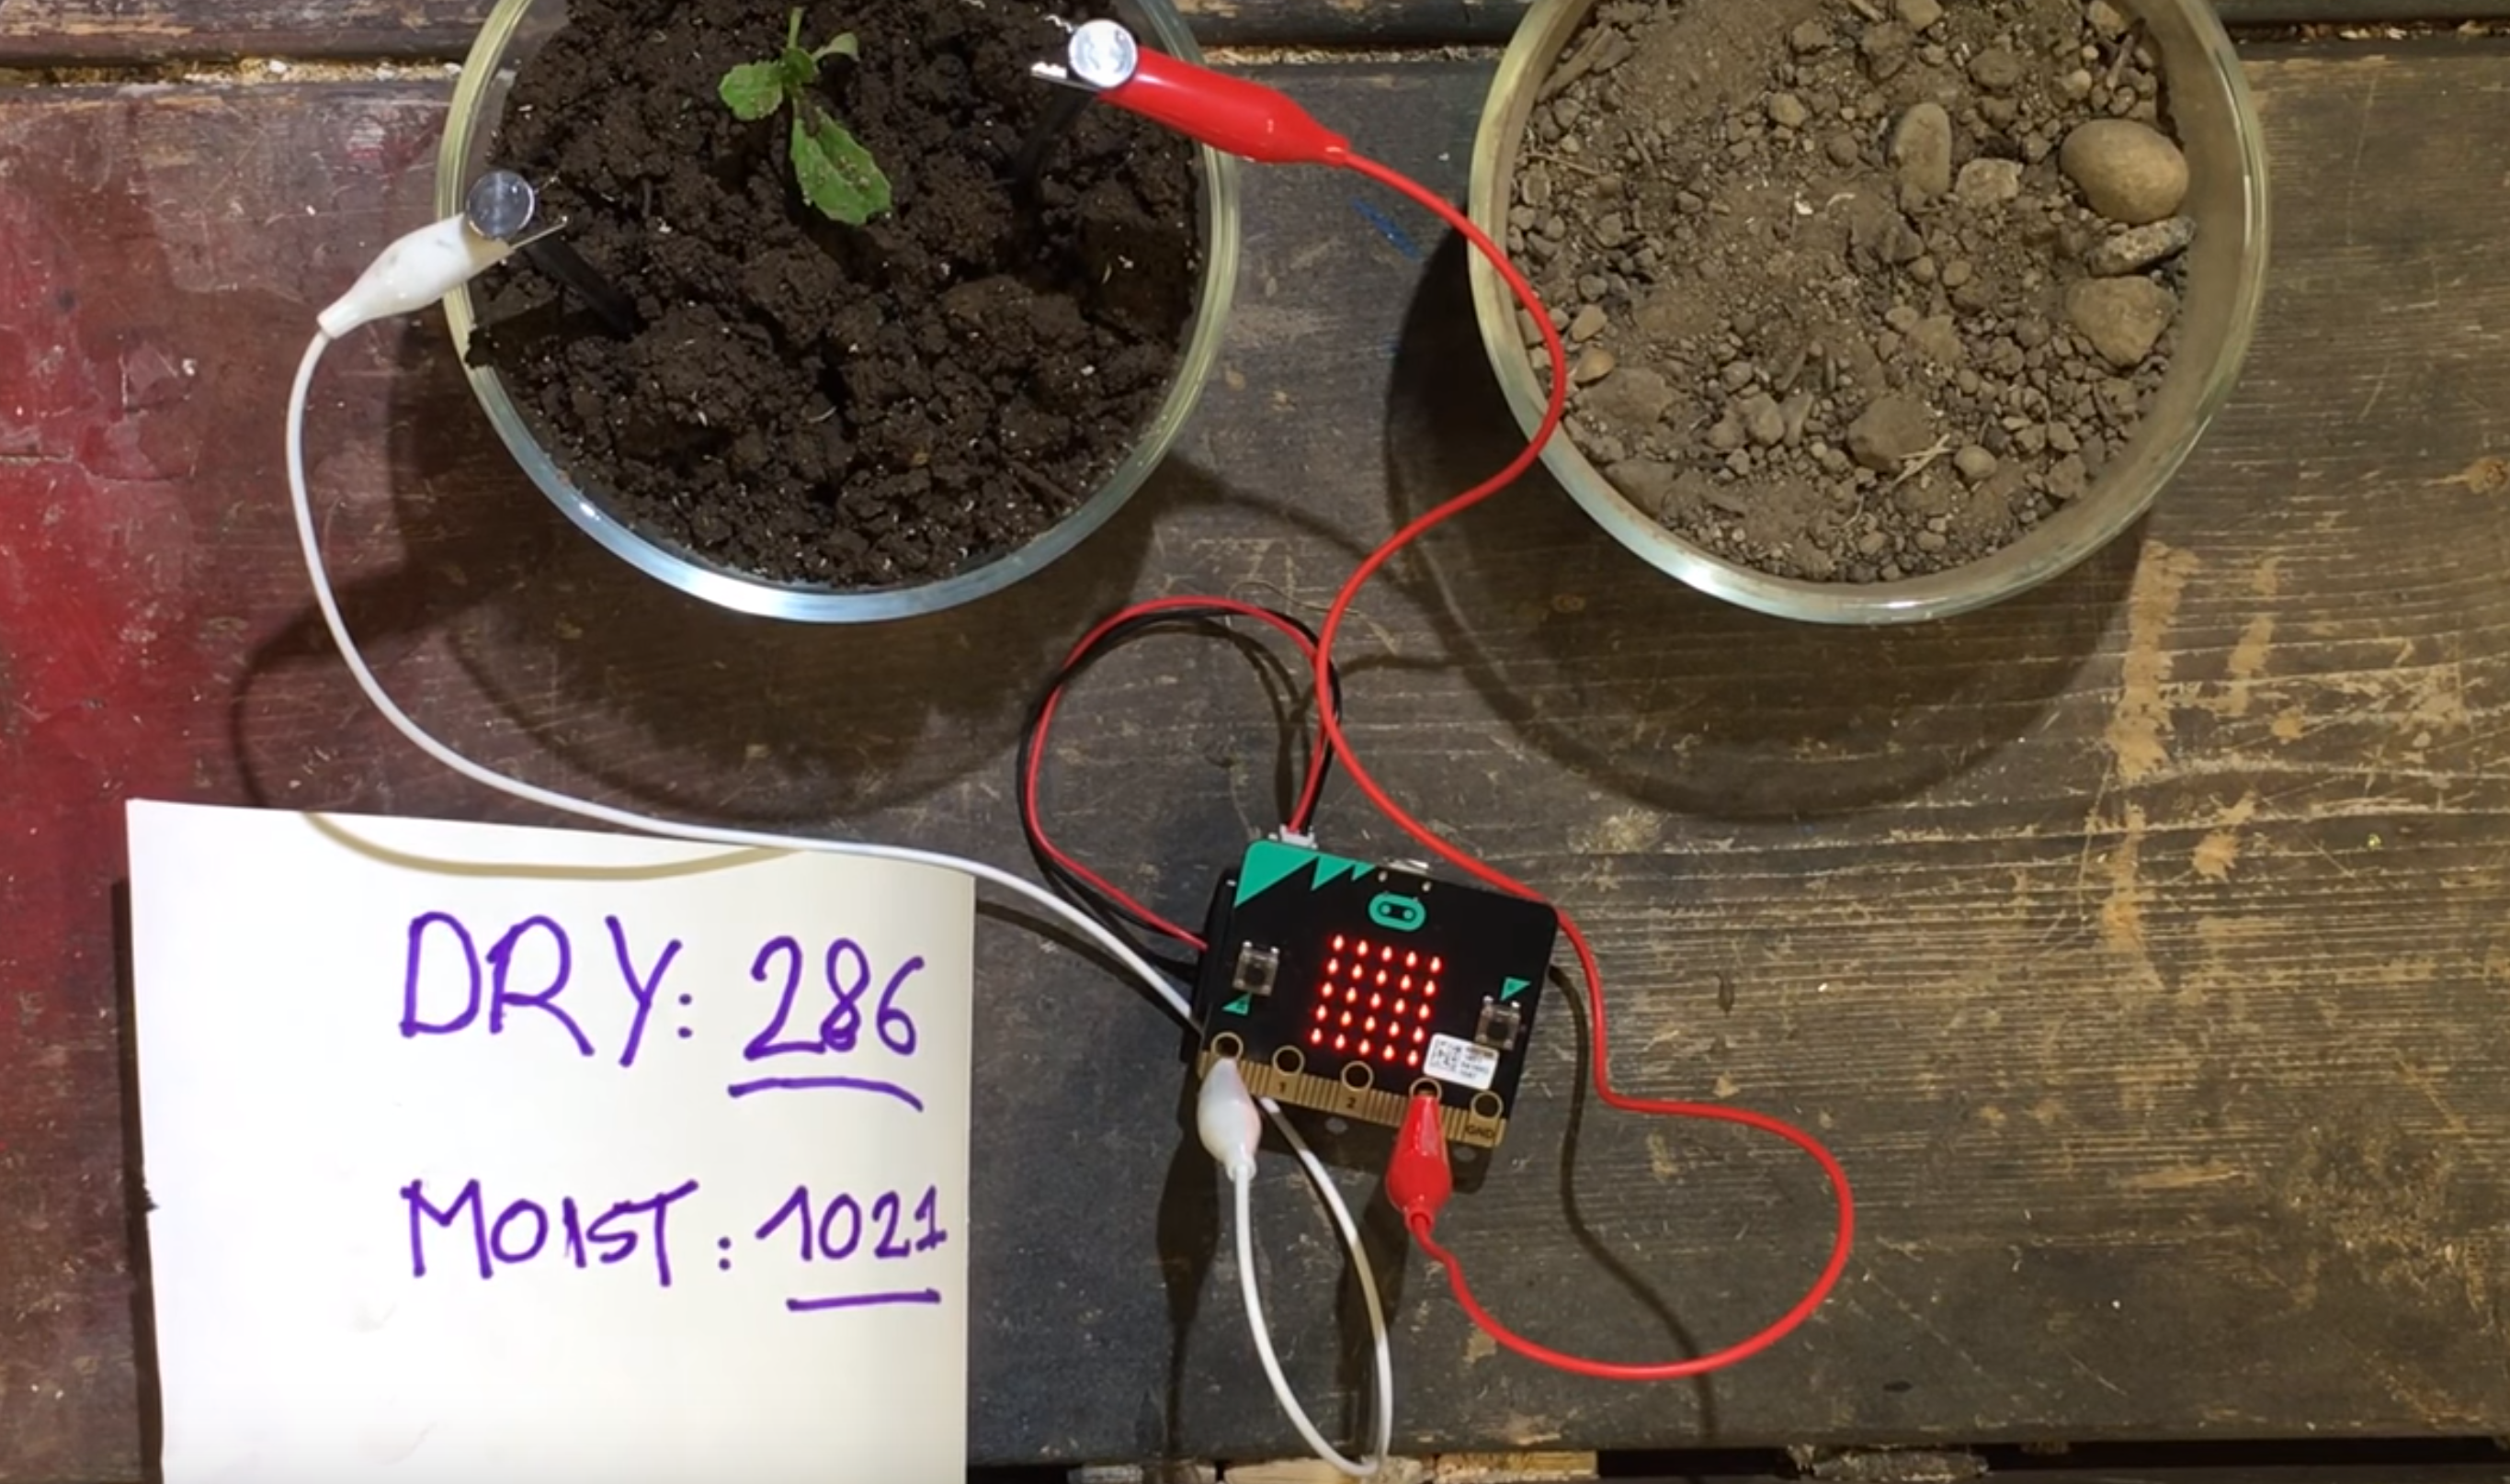
\includegraphics[width=3.3in]{images/moisture.jpg} 
    \includegraphics[width=3.3in]{images/moistureBlocks.png} 
    \caption{\label{fig:moisture}Measuring soil moisture via micro:bit pins.}
\end{figure}

Figure~\ref{fig:moisture} shows an environmental project that uses the 
micro:bit to measure soil moisture. The combination of water 
and soil nutrients makes the soil have some conductivity. The more water there is
in the soil, the greater its conductivity, which can be measured using
the analog pin API. In this project, the student
first learns to calibrate the measurement readings using dry and wet 
soil samples.  Then, the micro:bit is coded to periodically record the
reading. Using the micro:bit's Bluetooth radio, the readings also can
be sent to a central source.  In this way, the moisture of a set of soil
samples (in a classroom) can be recorded and reported. For more about this
project, see:
\begin{center}    
    \small{\url{makecode.microbit.org/projects/soil-moisture}}
\end{center} 

\begin{figure}[t]
\begin{verbatim}
  input.onButtonPressed(Button.A, () => {
    radio.sendString("H");
  });

  input.onButtonPressed(Button.B, () => {
    radio.sendString("S");
  });

  radio.onDataReceived(() => {
    let data = radio.receiveString();
    if (data == "H") {
      basic.showIcon(IconNames.Happy)
    } else if (data == "S") {
      basic.showIcon(IconNames.Sad)
    } else {
      basic.showString("?");
    }
  });
\end{verbatim}
\caption{\label{fig:mood}. Broadcasting simple messages using the micro:bit radio.}
\end{figure}

\subsection{Network}

Using a lower level of the Bluetooth stack, the micro:bit supports 
a simple radio broadcast protocol that can be used to send short messages
to a set of micro:bits. Figure~\ref{fig:mood} presents a simple example 
in JavaScript that shows how to use a micro:bit to communicate your 
``mood'' to other micro:bits in the vicinity.
Note that the micro:bit that sends a message does not
receive that message. 

The following two projects use the micro:bit radio to illustrate
how fireflies synchronize their blinking and how infections spread:
\begin{center}    
    \small{\url{makecode.microbit.org/projects/fireflies}}
\end{center}
\begin{center}    
    \small{\url{makecode.microbit.org/projects/infection}}
\end{center}

\subsection{Control}

The micro:bit can be attached to external actuators, such as servos,
to create systems that respond physically to their environment. 

% light sensor and servo
% https://makecode.microbit.org/projects/milk-carton-robot


